\subsection{\acrshort{orb}}\label{sec:orb_stats}
\begin{figure}[H]
\begin{subfigure}[t]{0.45\linewidth}
    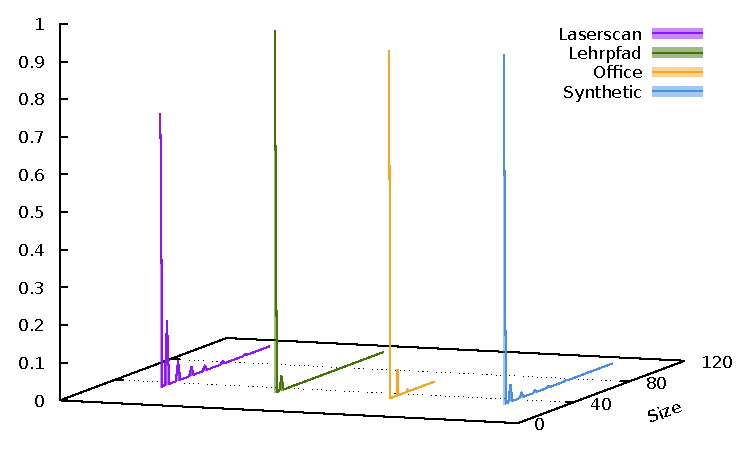
\includegraphics[width=\linewidth]{chapter06/results/ORB/flexion/size.pdf}%
    \caption{\gls{flexion-image}}
\end{subfigure}\quad
\begin{subfigure}[t]{0.45\linewidth}
    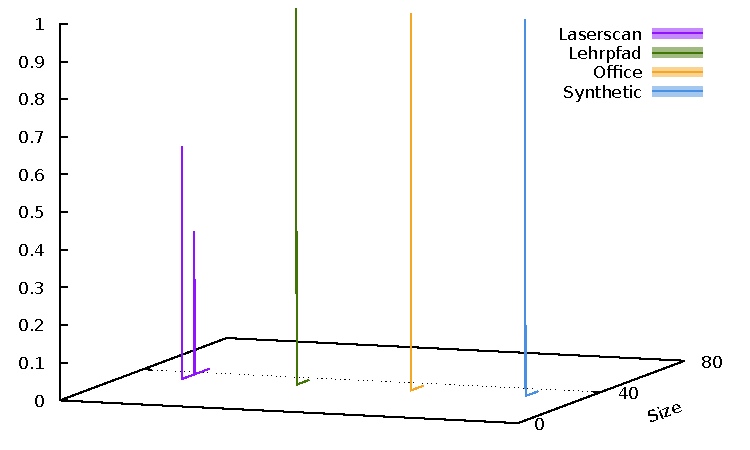
\includegraphics[width=\linewidth]{chapter06/results/ORB/bearing/size.pdf}
    \caption{\gls{bearing-angle-image}}
\end{subfigure}
\begin{subfigure}[t]{0.45\linewidth}
    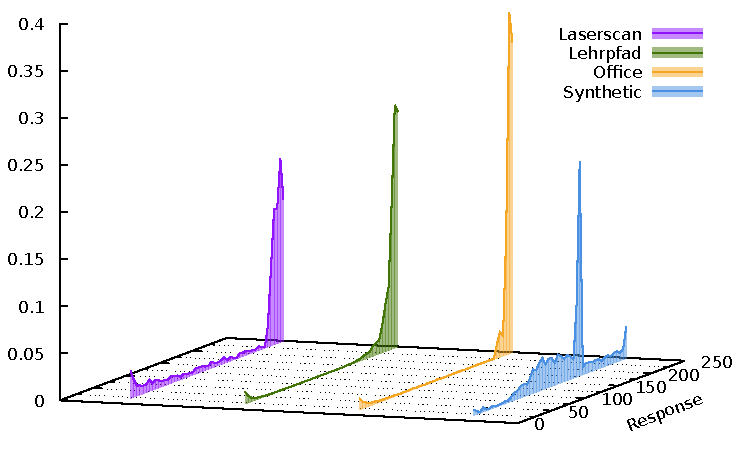
\includegraphics[width=\linewidth]{chapter06/results/ORB/flexion/response.pdf}%
    \caption{\gls{flexion-image}}
\end{subfigure}\quad
\begin{subfigure}[t]{0.45\linewidth}
    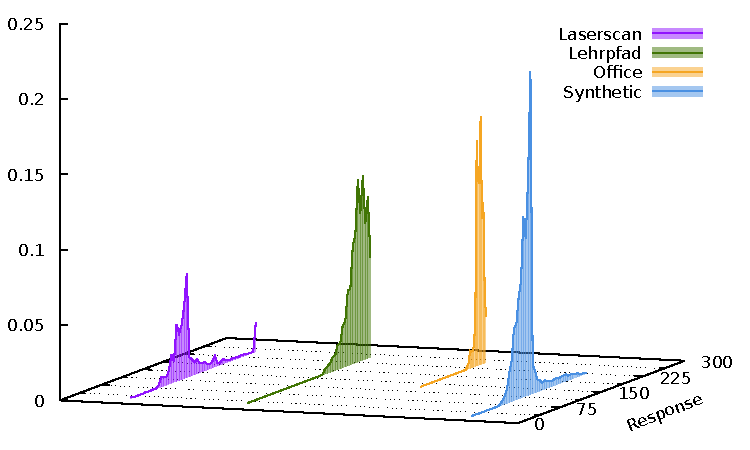
\includegraphics[width=\linewidth]{chapter06/results/ORB/bearing/response.pdf}
    \caption{\gls{bearing-angle-image}}
\end{subfigure}
    \caption{Overview of keypoint sizes and responses for the \acrshort{orb} detector.}
\end{figure}
\begin{figure}[H]
    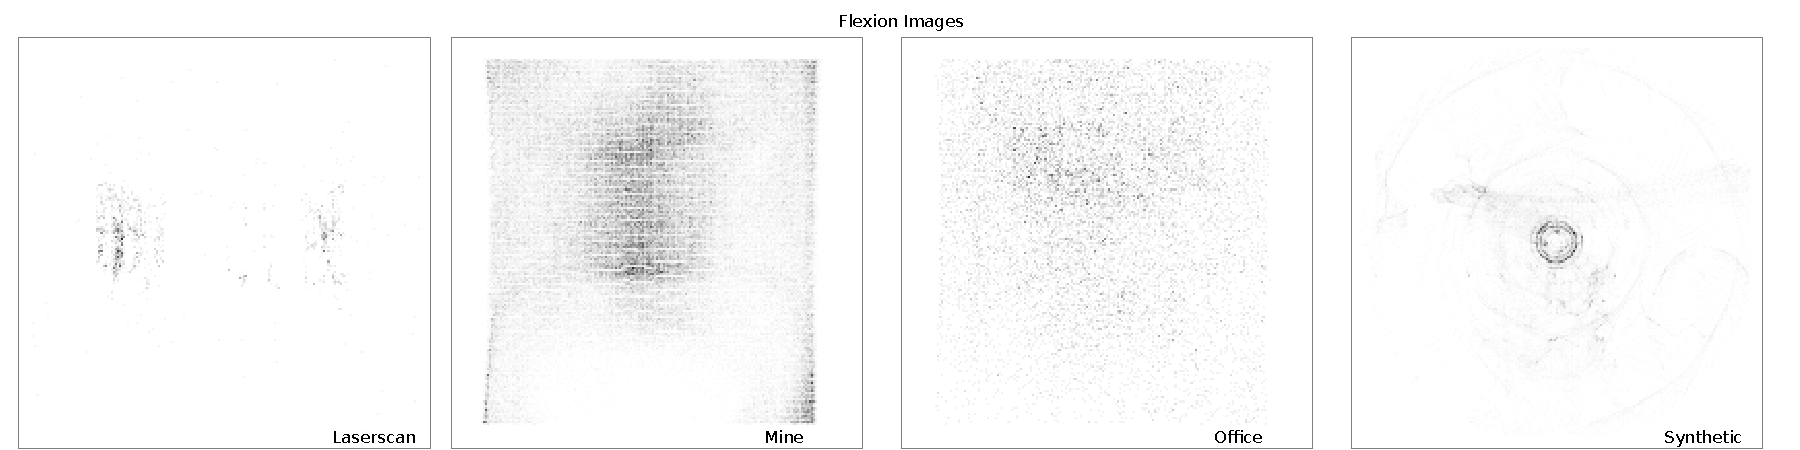
\includegraphics[width=\linewidth]{chapter06/results/ORB/flexion/distribution.pdf}\\
    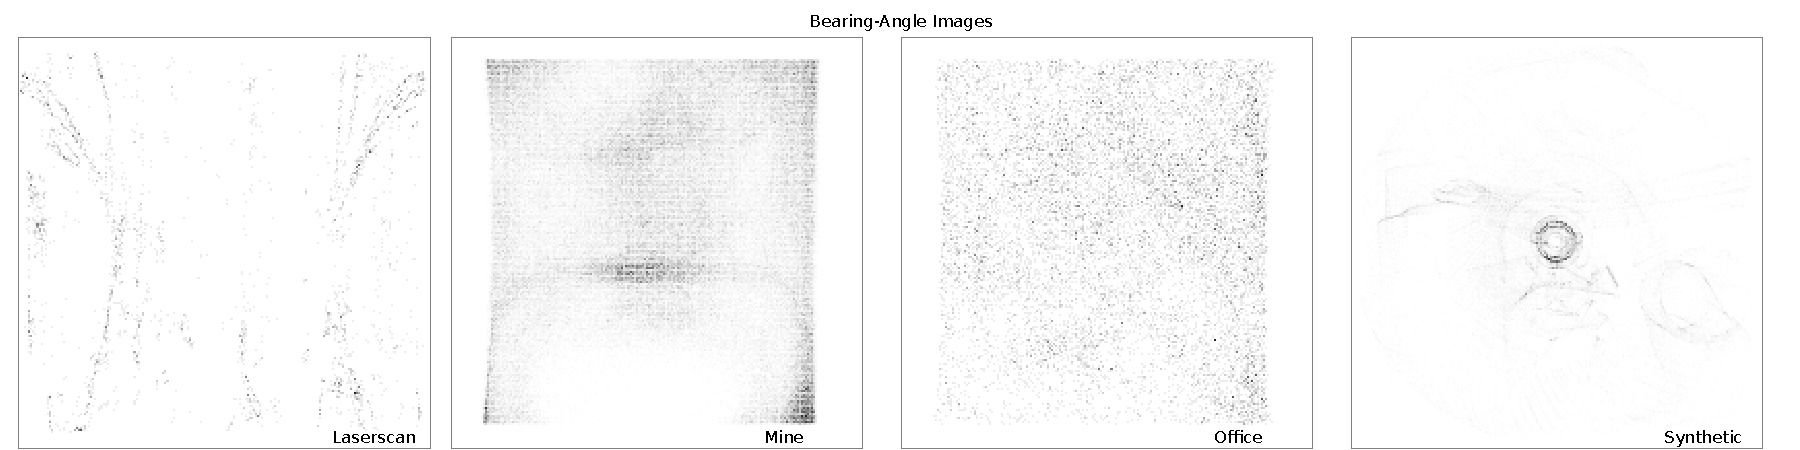
\includegraphics[width=\linewidth]{chapter06/results/ORB/bearing/distribution.pdf}%
    \caption{Keypoint distribution for the \acrshort{orb} detector.}
\end{figure}
